\subsubsection{Breakoutboards til \IIC sensorer}

Som temperatur- og luftfugtighedssensor er valgt \textit{HONEYWELL S\&C  HIH6030-021-001}, der kan måle både temperatur og luftfugtighed og har en \IIC grænseflade. Lyssensoren hedder \textit{Intersil ISL29010IROZ} og har ligeledes \IIC grænseflade. Følsomheden på denne kan indstilles til forskellige intervaller, fx 0-128000 lux, hvilket er passende for vores behov. Begge sensorer er forholdsvis små og vi har derfor behov for at lave breakoutboards til dem. Designet af disse er vist på Figur \ref{fig:temp_luftfugt_design}.

\begin{figure}[h]
\centering
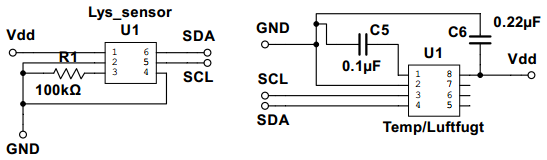
\includegraphics[width={\textwidth-6cm}, trim=0 0 0 0, clip=true]{../fig/TempOgLys.png}
\caption{Design af temp/luftfugtsensor og lyssensor breakoutboards.}
\label{fig:temp_luftfugt_design}
\end{figure}

Størrelserne på modstande og kondensatorer er fundet i de respektive datablade \cite{lib:TempHum_DS} og \cite{lib:LightSens}.